\chapter{Methods}
The study of cosmic objects, such as galaxies, relies on the analysis of the electromagnetic spectrum emanating from these distant sources. Within a spectrum, various pieces of information can be extracted, with the primary focus being on the intensity of light across a range of energies or frequencies. A crucial aspect of a spectrum involves determining the intensity at specific wavelengths.

This thesis will concentrate on utilizing specific information derived from spectra (e.g., flux, flux error) associated with both permitted and forbidden emission lines. In a galactic context, particularly within a galaxy cluster, the continuum originates from the diffuse light emitted by stars. On the other hand, emission lines, which are prominently observed in such environments, are typically generated by elements like Hydrogen, Helium, Oxygen, etc.

There are various methods to investigate the electromagnetic spectrum, with the two primary branches being Spectroscopy and Photometry.

Astrophysical spectroscopy is a fundamental tool used to analyze the electromagnetic radiation emitted or absorbed by celestial objects. By examining the spectral lines and features, it is possible to mine important informations such as chemical composition, temperature, density etc.

On the other hand, photometry measures the overall brightness of celestial objects across different wavelength bands, providing information about the spectral distribution of their luminous emission. 

In this Thesis Work i'll be focusing on a Spectroscopic study involving the fluxes of the Forbidden Emission lines of the spectrum.

\section{Data Description}
This thesis presents results obtained through the cross-matching of three distinct celestial catalogues:
\begin{itemize}
	\item\textbf{SDSS DR7 :} Our Main Catalogue of galaxies
	\item \textbf{C4-BCG :} The BCG Catalog 
	\item \textbf{Radio Emitters :}  The survey chosen for RadioLoud identification
\end{itemize}

\subsection{SDSS DR7}
The SDSS project, or Sloan Digital Sky Survey, is a comprehensive astronomical survey that maps the universe by capturing images, spectra, and photometric data of celestial objects over a large area of the sky. \cite{2009ApJS..182..543A}

Funding for the project has been provided by the Alfred P. Sloan Foundation, the Participating Institutions, the National Aeronautics and Space Administration, the National Science Foundation, the U.S. Department of Energy, the Japanese Monbukagakusho, and the Max Planck Society.

This ambitious project marked its beginnings in 2000 with the goals of obtaining CCD imaging in five broad bands, covering an area of $10,000 \, \text{deg}^2$ of high latitude sky and spectroscopy data of a million galaxies and over 100'000 quasars over the same area.

Observations have been conducted using a a dedicated wide-field 2.5 m telescope (Gunn
et al. 2006) located at Apache Point Observatory (APO) near Sacramento Peak in Southern New Mexico.

The telescope employs two distinct instruments. The first is a wide-field imager equipped with 24 tiles, each containing a 2048x2048 CCD. Imaging is performed along great circles at the sidereal rate, leading to exposure times of 54.1 seconds.

The astrometry is good to 45 milliarcseconds (mas) rms per coordinate at the bright end, while the photometric calibration is made in two modalities, respectively by tying to standard reference stars and by using the overlap between adjacent imaging runs in a process called ubercalibration.

Spectra are extracted and calibrated in terms of wavelength and flux. For galaxies near the main sample flux limit, the typical signal-to-noise ratio (S/N) is 10 per pixel. The broadband spectrophotometric calibration exhibits an accuracy of $4\%$ root mean square (rms) for point sources (Adelman-McCarthy et al. 2008), and the wavelength calibration is precise to $2 \, \text{km s}^{-1}$.

The SDSS data have been made public in a series of yearly data releases, This thesis works based its results from a galactic sample derived from "Data Release 7" by the Max Planck Institute for Astrophysics and Johns Hopkins University ( MPA-JHU )  teams, containing the derived properties of a total of 927'552 galaxy spectra.

\textbf{Physical Properties of interest :}
\begin{itemize}
		\item \textbf{Line Flux :}Flux from Gaussian fit to continuum subtracted data, corrected for foreground (galactic) reddening using techniques developed by O'Donnell \cite{1994ApJ...422..158O}
		\item \textbf{Error Line Flux :} Developed by analyzing the duplicate observations of galaxies, to compare the empirical spread in value determinations with the random errors.

\end{itemize}

\textbf{NOTA : Aggiungo un plot scat delle zone coperte da SDSS ?}


\subsection{C4 BCG Catalogue}
The identification of BCGs within our primary galaxy sample, previously described, relies on the findings of A. Von der Linden et al. \cite{2007MNRAS.379..867V, 2009yCat..73790867V}. These findings were derived from a subsequent analysis of the C4 Galaxy Cluster Catalog, initially developed by Miller et al. in 2005 \cite{2005AJ....130..968M}.

The C4 catalog comprises 748 galaxy clusters identified in the Second Data Release (DR2) of the Sloan Digital Sky Survey (SDSS). Utilizing a seven-dimensional position and color space, the C4 cluster-finding algorithm identifies overdensities. 

Covering approximately 2600 square degrees of the sky, the catalog spans redshifts from about 0.02 to 0.17. It includes various properties like sky location, mean redshift, galaxy membership, optical luminosity (Lr), velocity dispersion, and measures of substructure and large-scale environment.

This catalog represents one of the initial cluster catalogs constructed directly from SDSS spectroscopic data, addressing issues related to projection effects and employing mock galaxy catalogs derived from realistic N-body simulations to analyze the clustering algorithm's parameters and improve its completeness.

In this context, the work by Von Der Linden et al.  \cite{2007MNRAS.379..867V} is noteworthy, as it builds upon the C4 catalog but introduces improved algorithms for BCG identification and measuring cluster velocity dispersion,  ultimately yielding a sample of 625 BCGs.

Correcting for the SDSS photometric pipeline's tendency to underestimate luminosities in dense environments, the research refines the C4 galaxy cluster sample, addressing issues related to BCG luminosity underestimation. Given the challenges with SDSS photometry, especially for large galaxies in crowded areas, the study avoids using magnitude measurements assuming a specific profile shape.

The C4 catalog provides potential BCG candidates, but approximately $30\% $ of clusters miss the true BCG due to fiber collisions. To address this issue,  Von der Linden's team developed an algorithm to identify the BCG by estimating the virial radius, selecting the two brightest galaxies within the mean galaxy's projection, and assessing criteria such as concentration index, color compatibility, and redshift.

\subsection{The Radio Catalogue}
To investigate the radio emission characteristics of both BCGs and non-BCGs, this study conducted a crossmatch between the primary SDSS sample and a dataset comprising 2,712 radio-luminous galaxies from the work by \cite{2005MNRAS.362....9B}. This collection of radio-luminous objects resulted from a complex cross-matching process involving the main spectroscopic galaxy sample and two radio surveys: the National Radio Astronomy Observatories (NRAO) Very Large Array (VLA) Sky Survey (NVSS) \cite{1998AJ....115.1693C} and the Faint Images of the Radio Sky at Twenty centimeters (FIRST) survey. \cite{1995ApJ...450..559B}

The NVSS was the first radio survey with a sufficiently high angular resolution (45 arcsec) to allow automated cross-correlation with optical surveys. However, the FIRST catalogue offers superior angular resolution (approximately 5 arcsec), resulting in samples with much higher reliability. Nonetheless, the high angular resolution of FIRST presents its own challenges, as it is insensitive to extended radio structures and resolves out the extended emission of radio sources. Consequently, the total radio luminosity of sources larger than a few arcseconds is systematically underestimated by FIRST. To address these limitations, a hybrid approach utilizing both NVSS and FIRST surveys has been developed to identify radio sources associated with galaxies in the SDSS spectroscopic sample. This approach capitalizes on the sensitivity of NVSS to large-scale radio structures and the high angular resolution of FIRST to reliably pinpoint the host galaxy.

The obtained radio source sample demonstrated a completeness of $95\%$ and a reliability of $98.9\%$, upgradingo the achievable performance of each individual survey. The sample was subsequently classified into two groups: radio-loud active galactic nuclei (AGN) and galaxies where radio emission is predominantly driven by star formation. Classification was based on a galaxy's position in the 4000-Å break strength versus radio luminosity per unit stellar mass plane, resulting in a dataset of 2,215 radio-loud AGN and 497 star-forming galaxies with radio luminosity exceeding 5 mJy at 1.4 GHz.

\begin{figure}[b]
  \centering
  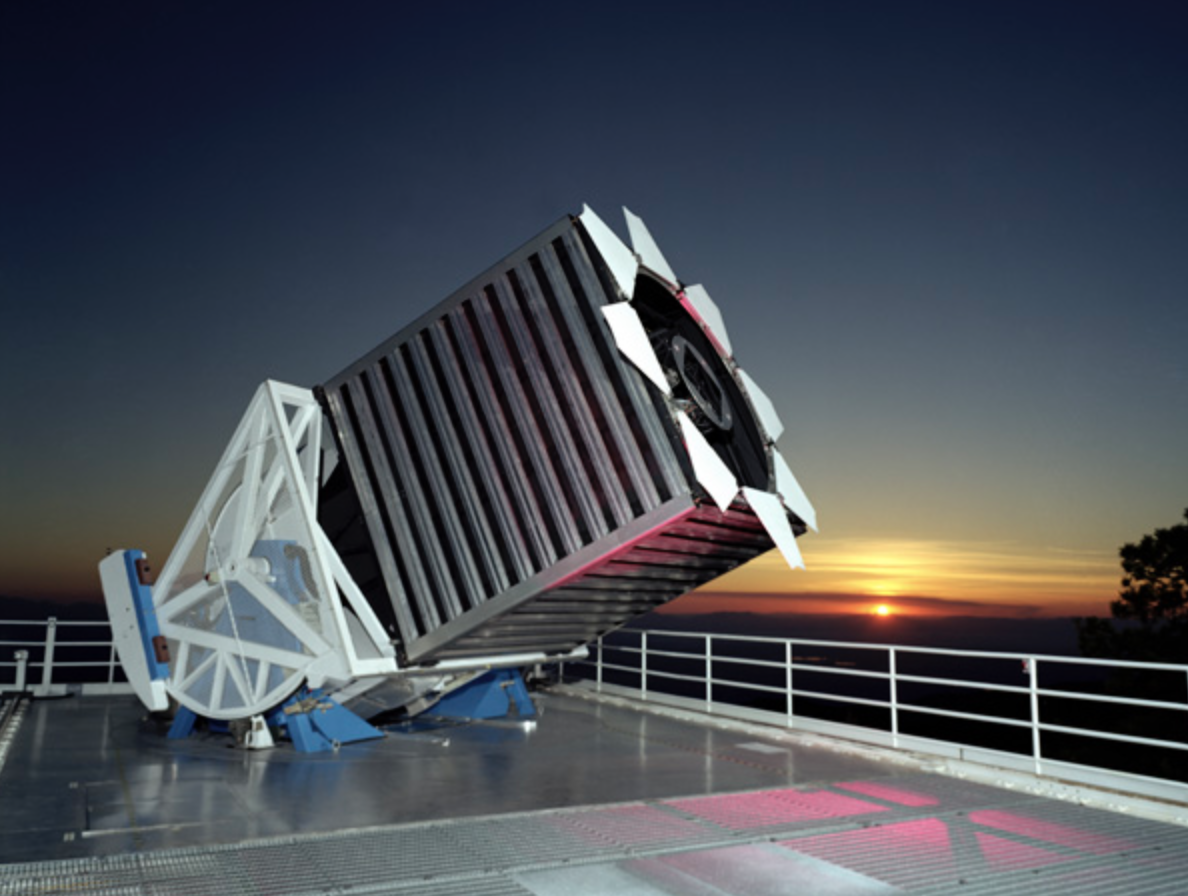
\includegraphics[width=0.55\textwidth]{SDSS}
  \caption{The main 2.5-meter SDSS Telescope }
  \label{3}
\end{figure}


\newpage
\section{Data Analysis}
How we analyzed the data, where do we defined the fractions calculated ?
\subsection{Optical analysis}
Describe each population of the BPT diagram and its peculiarities, before starting the description of how we collected and processed the data to finally create BPT diagrams .
Finally there's the need to explain how we interpreted the diagrams to finally calculate the fractions ( in this case you need to explain which algorithm has been chosen and why ) 


\subsection{Radio Analysis}
I certainly need to focus on how i have chosen the range of identification, to recognize which element of sdss was effectively recognized as a Radioloud.

Following to this it is necessary to explain how we selected the elements in which define the fractions, by selecting elements of SDSS nearby the location in which best et al finds mostly its radio-emitting elements!